% Section content template for individual Educative lessons
% This file contains the actual content for a specific section
% Generated from Educative API section content

% Section: Challenges of Google Maps' Design
% Section ID: 4659727862071296
% Section Slug: challenges-of-google-maps-design
% Generated: 2025-12-07T23:06:09.554248

\subsection{Meeting the challenges}\label{TuAkuVwJVKpzgtChrWw_I}
\\
We listed two challenges in the \href{https://www.educative.io/courses/grokking-the-system-design-interview/requirements-of-google-maps-design\#Challenges}{Introduction} lesson: scalability and ETA computation. Let 's see how we meet these challenges.

\subsubsection{Scalability}\label{yGTaXDgk6ilZgqG-i0mfG}
\\
\textbf{Scalability} is about the ability to efficiently process a huge road network graph. We have a graph with billions of vertices and edges, and the key challenges are inefficient loading, updating, and performing computations. For example, we have to traverse the whole graph to find the shortest path. This results in increased query time for the user. So, what could be the solution to this problem?
\\
The idea is to break down a large graph into smaller subgraphs, or partitions. The subgraphs can be processed and queried in parallel. As a result, the graph construction and query processing time will be greatly decreased. So , we divide the globe into small parts called segments. Each segment corresponds to a subgraph.
\\
\paragraph{Segment}\label{GnRgIyzlLJhIYx5yrloQQ}
\\
A \textbf{segment} is a small area on which we can work easily. Finding paths within these segments works because the segment's road network graph is small and can be loaded easily in the main memory, updated, and traversed(Traversing is visiting the graph vertices to reach a specific vertex.). A city, for example, can be divided into hundreds of segments, each measuring \protect\phantomsection\label{katex_inline_YMGJVQGAtHE7KazGAMvvD}{{{\(5 \times 5\)}}} miles.
\begin{quote}
\textbf{Note}: A segment is not necessarily a square. It can also be a polygon. However, we are assuming square segments for ease of explanation.
\end{quote}
\\
Each segment has four coordinates that help determine which segment the user is in. Each coordinate consists of two values, the latitude and longitude.

\begin{figure}[htbp]
 \centering
 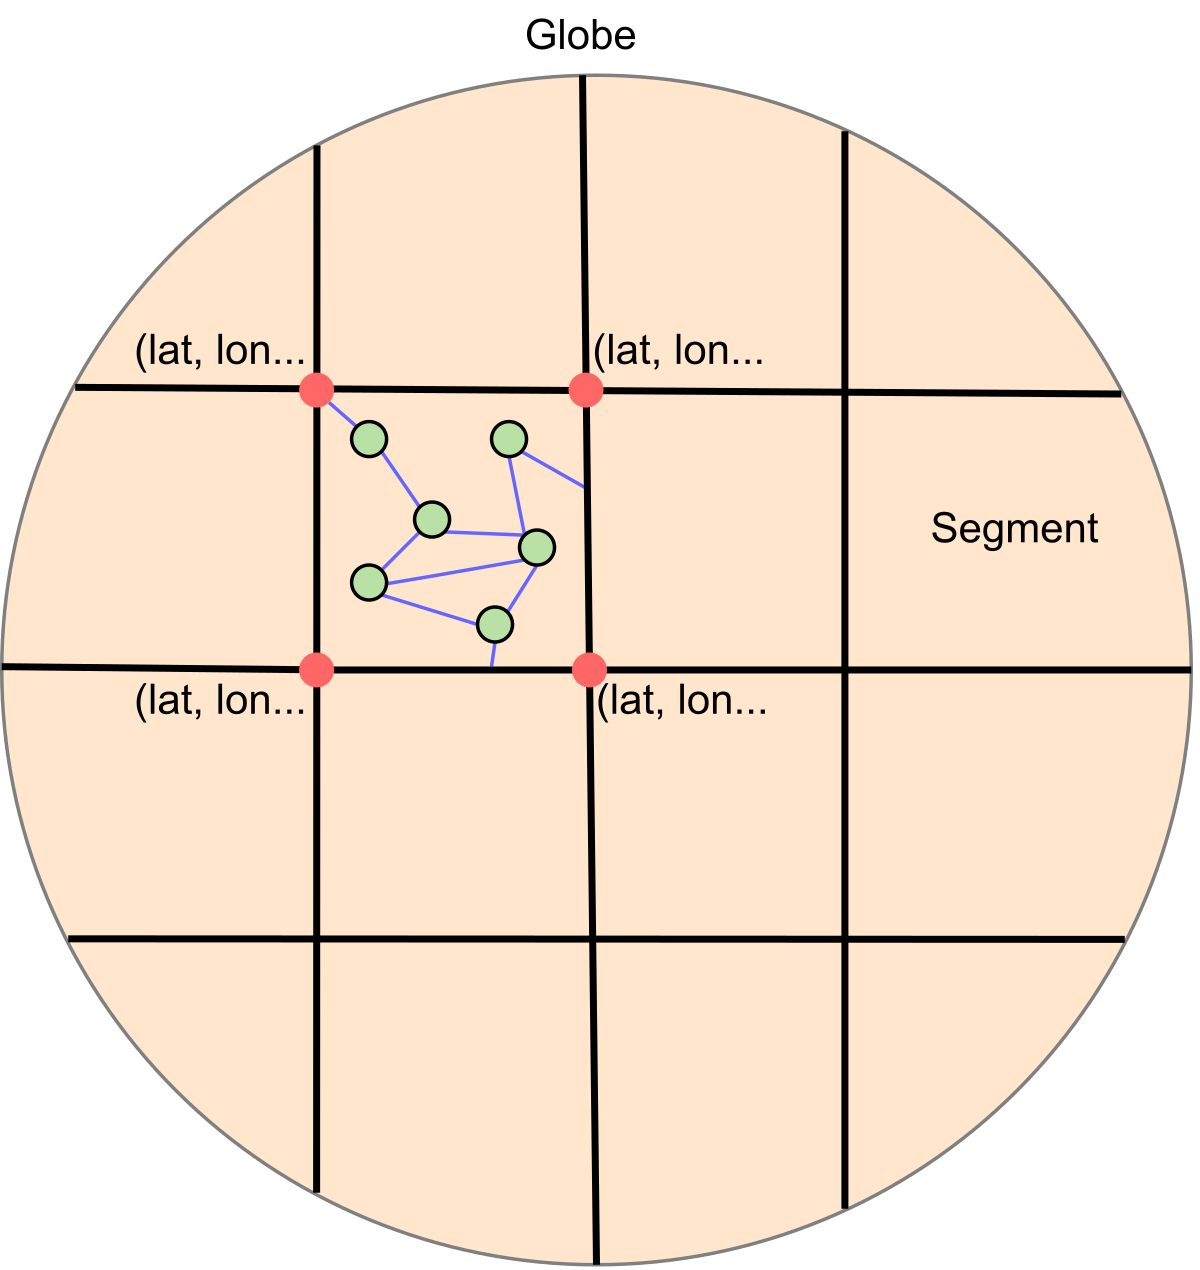
\includegraphics[width=0.25\textwidth]{Images/chapter_28/section_4659727862071296/5624646229819392.png}
 \caption{Partitioning the globe into small segments, and each segment has four coordinates with latitude and longitude values}
\end{figure}

Let's talk about finding paths between two locations within a segment. We have a graph representing the road network in that segment. Each intersection/junction acts as a vertex and each road acts as an edge. The graph is weighted, and there could be multiple weights on each edge---such as distance, time, and traffic---to find the optimal path. For a given source and destination, there can be multiple paths. We can use any of the graph algorithms on that segment's graph to find the shortest paths. The most common shortest path algorithm is \textbf{Dijkstra's algorithm}.

The traditional Dijkstra algorithm performs a guided search to find the shortest path. However, it comes at the cost of an increased query time. We have to set a limit on the query time because we wouldn't want the user to wait too long to get their results. So , we'll go with finding the optimal path within the given time cost.
\\
The \textbf{A}* algorithm is an extension of the Dijkstra algorithm that uses heuristics to guide its search. Instead of finding the shortest path, A* finds the optimal path that is calculated by minimizing the following function.
\\
\(f(n)=g(n)+h(n)\)
\\
Here, \(n\) is the next node on the path, \(g(n)\) is the cost of the path from the start node to \(n\), and \(h(n)\) is a heuristic function that estimates the cost of the cheapest path from \(n\) to the goal.
\begin{quote}
Note: There are some algorithms that are specifically designed for road networks that focus on achieving shorter query time. These algorithms are \href{https://arxiv.org/pdf/1603.01607.pdf}{A*}, \href{http://www.diag.uniroma1.it/challenge9/papers/kohler.pdf}{Arc flags}, \href{https://en.wikipedia.org/wiki/Contraction_hierarchies}{contraction hierarchies}, \href{https://www.researchgate.net/publication/6366597_Fast_Routing_in_Road_Networks_with_Transit_Nodes}{transit node routing}, \href{https://archive.siam.org/meetings/alenex04/abstacts/rgutman1.pdf}{reach-based routing}, and \href{https://www.microsoft.com/en-us/research/wp-content/uploads/2010/12/HL-TR.pdf}{hub labeling}.
\end{quote}

After running the shortest path algorithm on the segment's graph, we store the algorithm's output in a distributed storage to avoid recalculation and cache the most requested routes. The algorithm's output is the shortest distance in meters or miles between every two vertices in the graph, the time it takes to travel via the shortest path, and the list of vertices along every shortest path. All of the above processing (running the shortest path algorithm on the segment graph) is done offline (not on a user's critical path).

\begin{figure}[htbp]
 \centering
 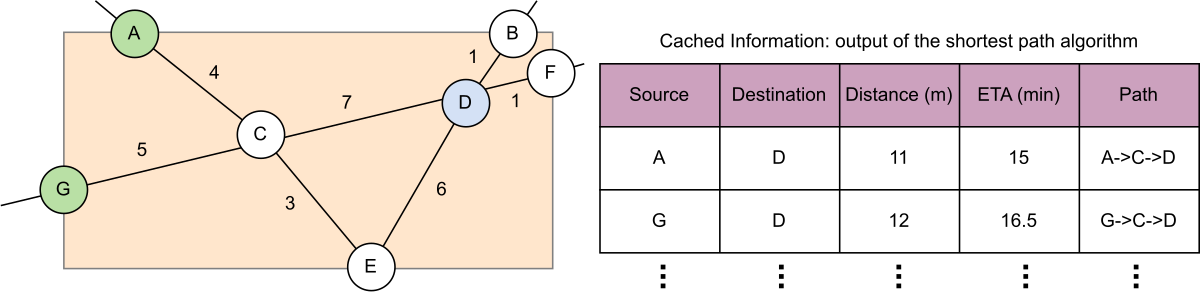
\includegraphics[width=0.5\textwidth]{Images/chapter_28/section_4659727862071296/5628801208025088.png}
 \caption{Finding a path between vertices within a segment}
\end{figure}

The illustration above shows how we can find the shortest distance in terms of miles between two points. For example, the minimum distance (\texttt{m}) between points A and D is 11 miles by taking the path A-\textgreater C-\textgreater D. It has an ETA of 15 minutes.
\\
We've found the shortest path between two vertices. What if we have to find the path between two points that lie on the edges? What we do is find the vertices of the edge on which the points lie, calculate the distance of the point from the identified vertices, and choose the vertices that make the shorter total distance between the source and the destination. The distance from the source (and destination) to the nearest vertices is approximated using latitude/longitude values.

\begin{figure}[htbp]
 \centering
 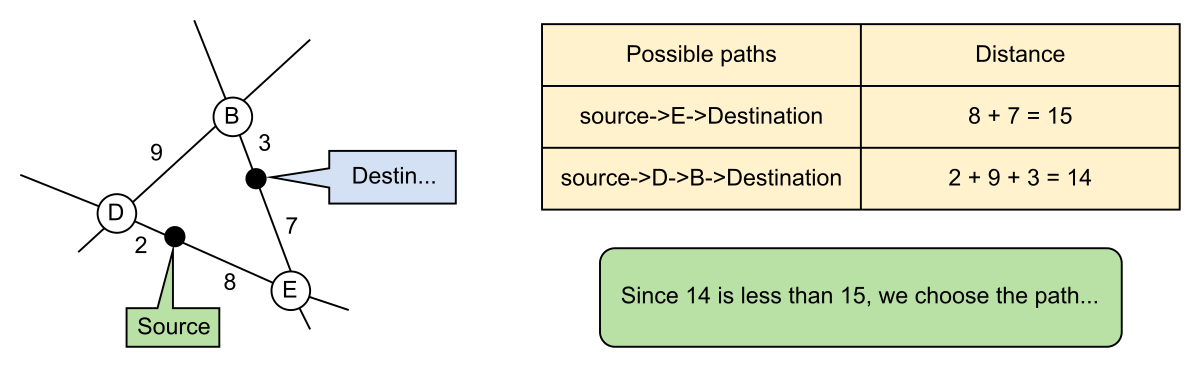
\includegraphics[width=0.5\textwidth]{Images/chapter_28/section_4659727862071296/4750278599639040.png}
 \caption{Choosing a path between points that lie on the edge}
\end{figure}

We're able to find the shortest paths within the segment. Let 's see what happens when the source and the destination belong to two different segments, and how we connect the segments.\\
\\
\paragraph{Connect two segments}\label{vdYSLeVa47s4WT5r1u1vn}
\\
Each segment has a unique name and boundary coordinates. We can easily identify which location (latitude, longitude) lies in which segment. Given the source and the destination, we can find the segments in which they lie. For each segment, there are some boundary edges, which we call \textbf{exit points}. In the illustration below, we have four exit points, S4E1, S4E2, S4E3, and S4E4.
\begin{quote}
\textbf{Note}: Besides the vertices we have inside the segment, we also consider the exit points of a segment as vertices and calculate the shortest path for these exit points. So for each segment, we calculate the shortest path between exit points in addition to the shortest path from the exit points to vertices inside the segment. Each vertex's shortest path information from the segment's exit points is cached.
\end{quote}

\begin{figure}[htbp]
 \centering
 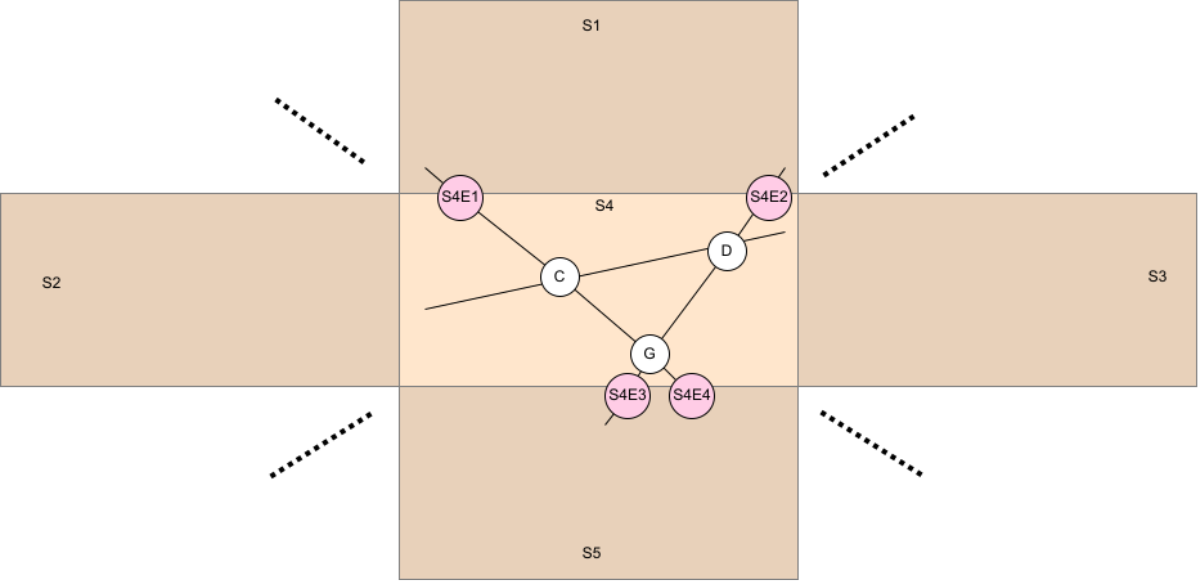
\includegraphics[width=0.5\textwidth]{Images/chapter_28/section_4659727862071296/5980966950797312.png}
 \caption{Connecting the segments by considering exit points of a segment as vertices}
\end{figure}

An exit point connects neighboring segments and is shared between them. In the illustration above, each exit point is connecting two segments and each is shared between two segments. For example, the exit point S4E1 is also an exit point for S1. Having all the exit points for each segment, we can connect the segments and find the shortest distance between two points in different segments. While connecting the segments, we don\textquotesingle t care about the inside segment graph. We just need exit points and the cached information about the exit points. We can visualize it as a graph made up of exiting vertices, as shown in the following illustration.

\begin{figure}[htbp]
 \centering
 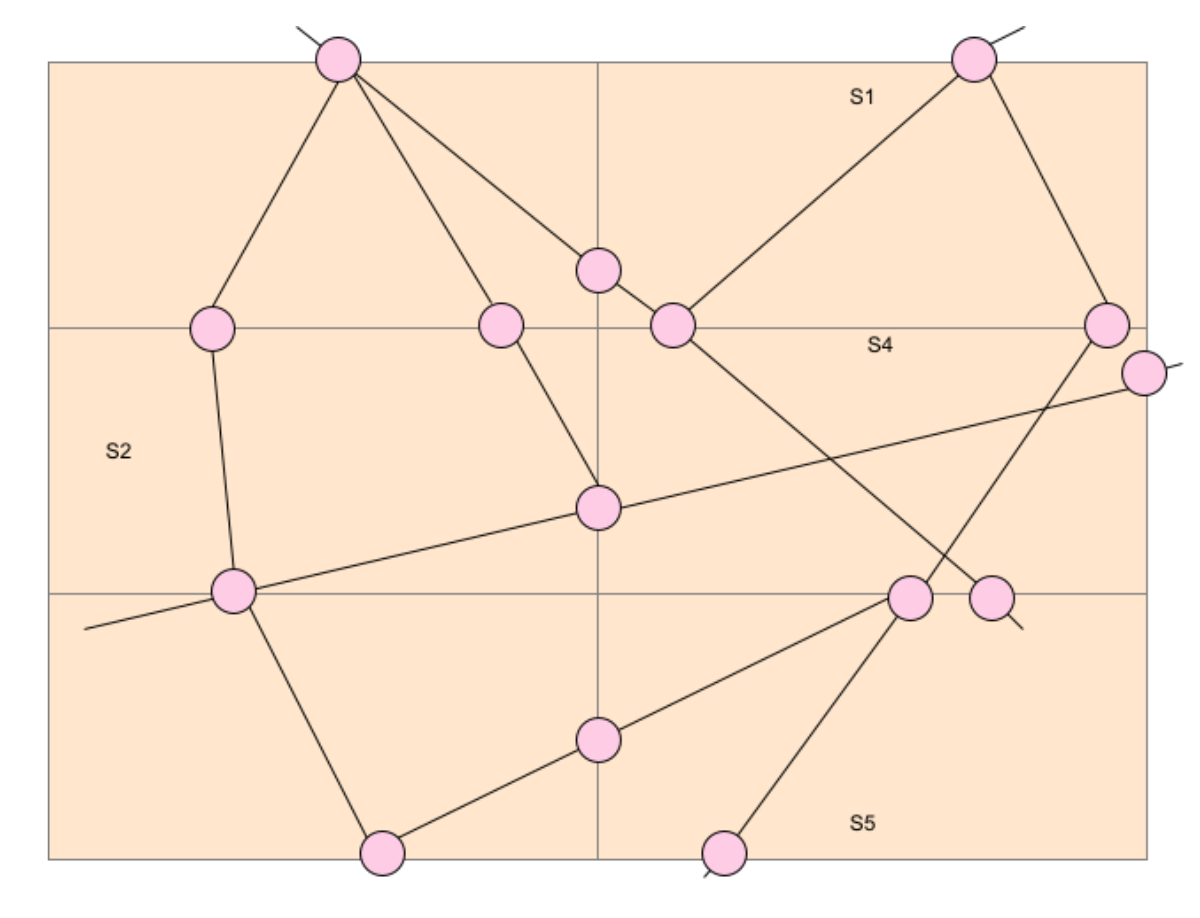
\includegraphics[width=0.5\textwidth]{Images/chapter_28/section_4659727862071296/4575587691921408.png}
 \caption{A graph made up of exit points, where the lines connecting the exit points are not actually straight. There could be many vertices in between the two exit points}
\end{figure}

Since we can't run the shortest path algorithm for all the segments throughout the globe, it's critical to figure out how many segments we need to consider for our algorithm while traveling inter-segment. The aerial distance(Aerial distance is the distance between two places measured in a straight line through the air rather than using roads on the ground.) between the two places is used to limit the number of segments. With the source and destination points, we can find the aerial distance between them using the \href{https://en.wikipedia.org/wiki/Haversine_formula}{haversine formula}.
\\
Suppose the aerial distance between the source and the destination is 10 kilometers. In that case, we can include segments that are at a distance of 10 kilometers from the source and destination in each direction. This is a significant improvement over the large graph.
\\
Once the number of segments is limited, we can constrain our graph so that the vertices of the graph are the exit points of each segment, and the calculated paths between the exit points are the graph's edges. All we have to do now is run the shortest path algorithm on this graph to find the route. The following illustration shows how we find the path between two points that lie in different segments.

\begin{figure}[htbp]
 \centering
 \begin{subfigure}[b]{0.48\textwidth}
 \centering
 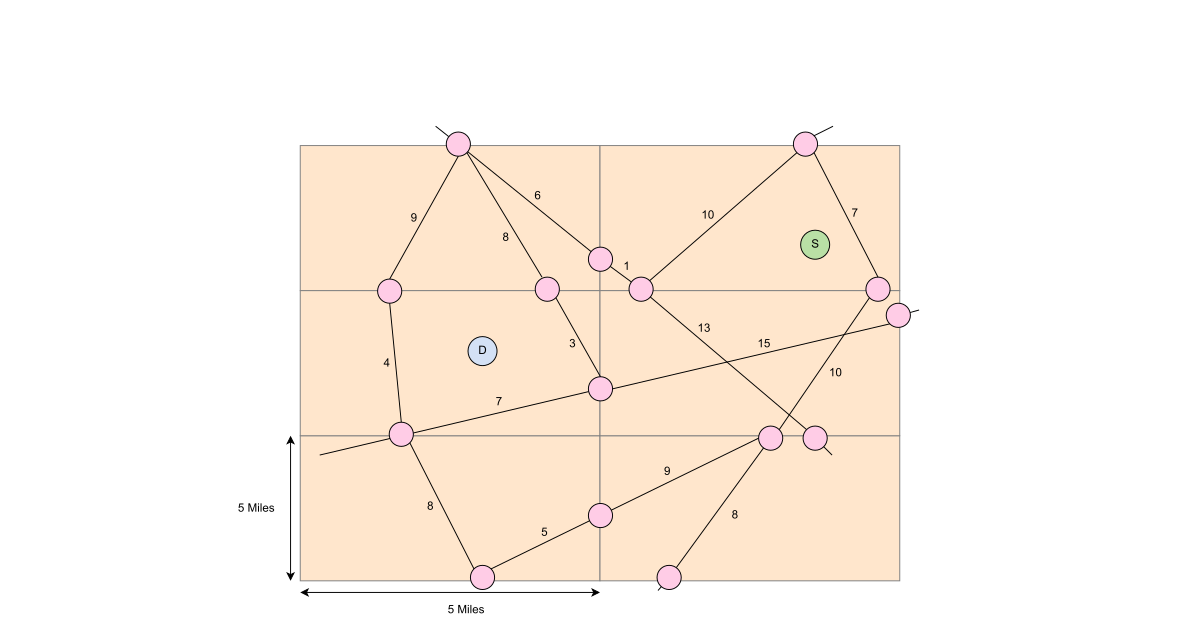
\includegraphics[width=\textwidth]{Images/chapter_28/section_4659727862071296/5566860162760704.png}
 \caption{Source S and Destination D lie in two different segments, and we have to find the shortest route between them}
 \end{subfigure}
 \hfill
 \begin{subfigure}[b]{0.48\textwidth}
 \centering
 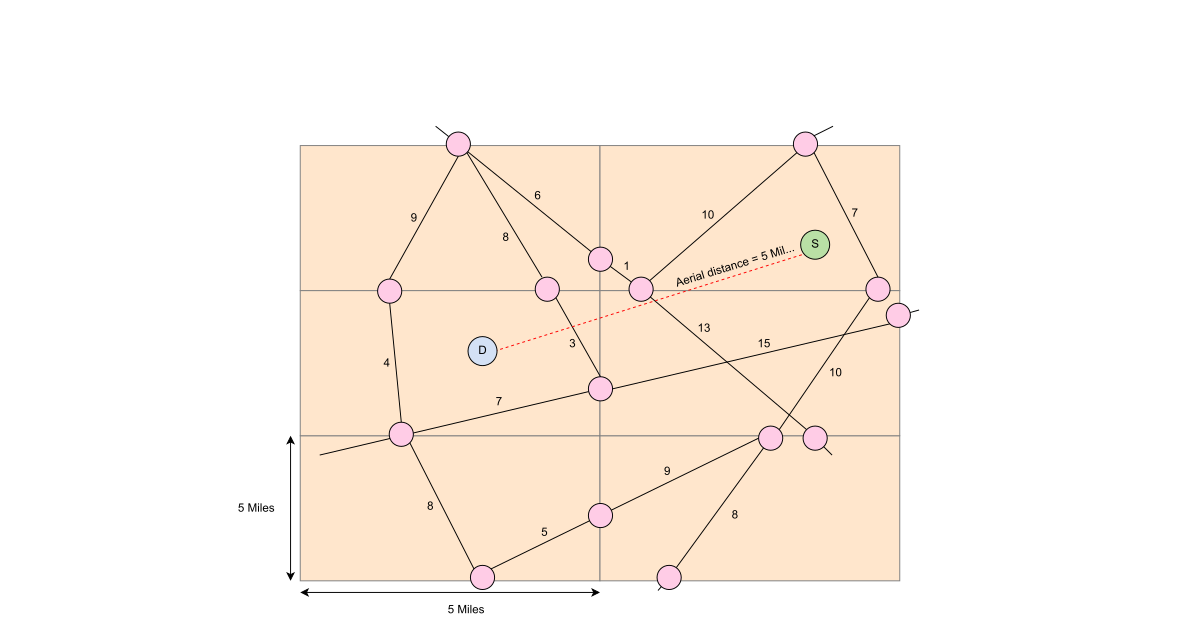
\includegraphics[width=\textwidth]{Images/chapter_28/section_4659727862071296/5637840369352704.png}
 \caption{We assume that the aerial distance between S and D is 5 miles, calcuated using the haversine formula}
 \end{subfigure}
\end{figure}

\begin{figure}[htbp]
 \centering
 \begin{subfigure}[b]{0.48\textwidth}
 \centering
 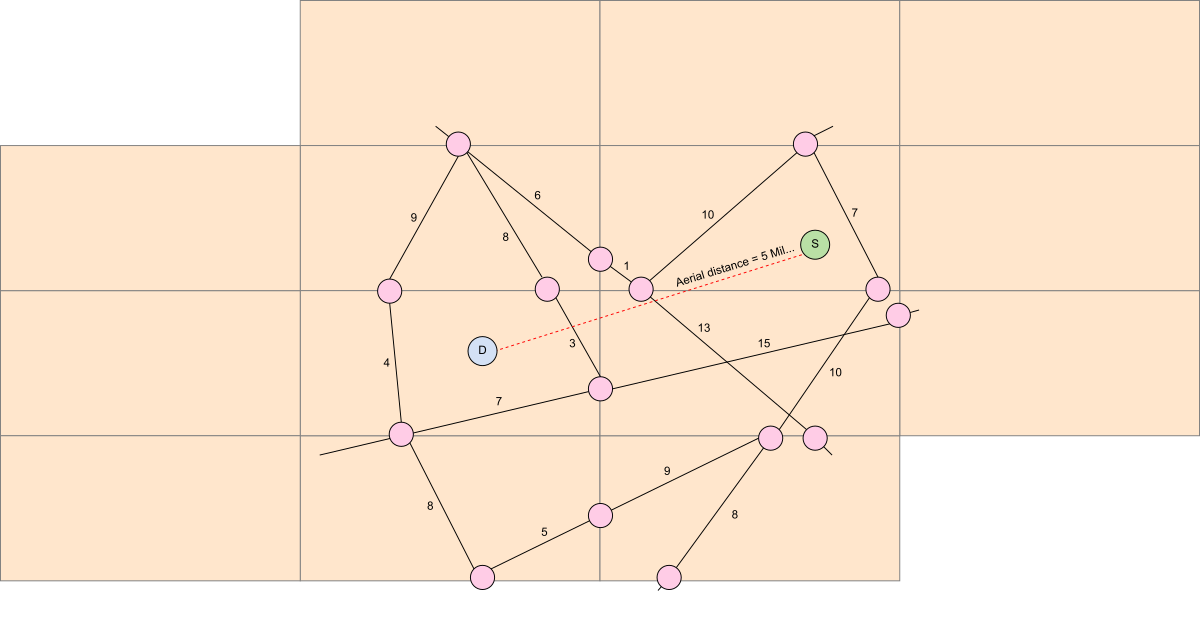
\includegraphics[width=\textwidth]{Images/chapter_28/section_4659727862071296/4705257812918272.png}
 \caption{Since the aerial distance is 5 miles, we include the segments that are at a 5-mile distance from S and D in all directions}
 \end{subfigure}
 \hfill
 \begin{subfigure}[b]{0.48\textwidth}
 \centering
 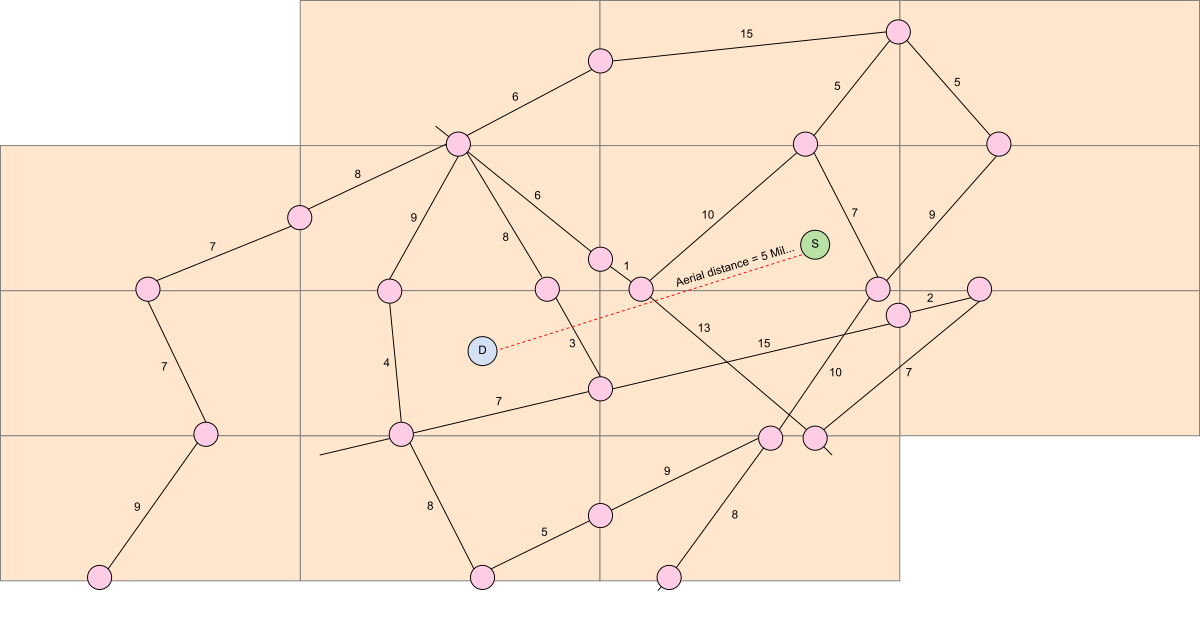
\includegraphics[width=\textwidth]{Images/chapter_28/section_4659727862071296/4624269158121472.png}
 \caption{Let’s include the exiting points of the new segments in the graph}
 \end{subfigure}
\end{figure}

\begin{figure}[htbp]
 \centering
 \begin{subfigure}[b]{0.48\textwidth}
 \centering
 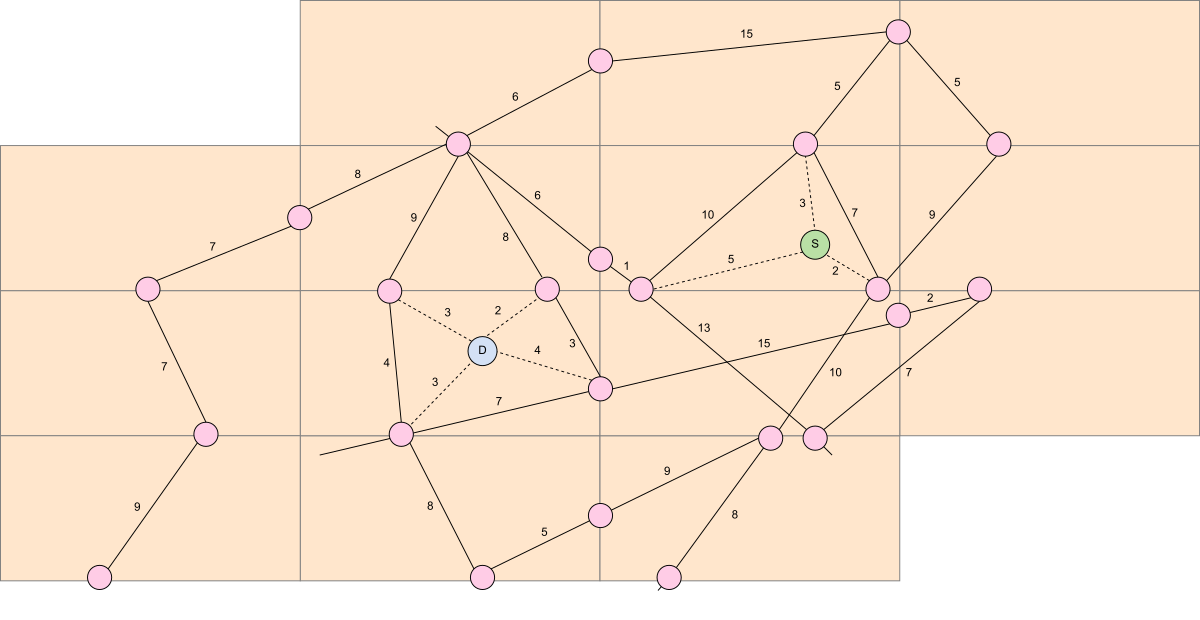
\includegraphics[width=\textwidth]{Images/chapter_28/section_4659727862071296/5436432013590528.png}
 \caption{Find the possible exits for S and D from their respective segments and the shortest path (already calculated) to all exit points}
 \end{subfigure}
 \hfill
 \begin{subfigure}[b]{0.48\textwidth}
 \centering
 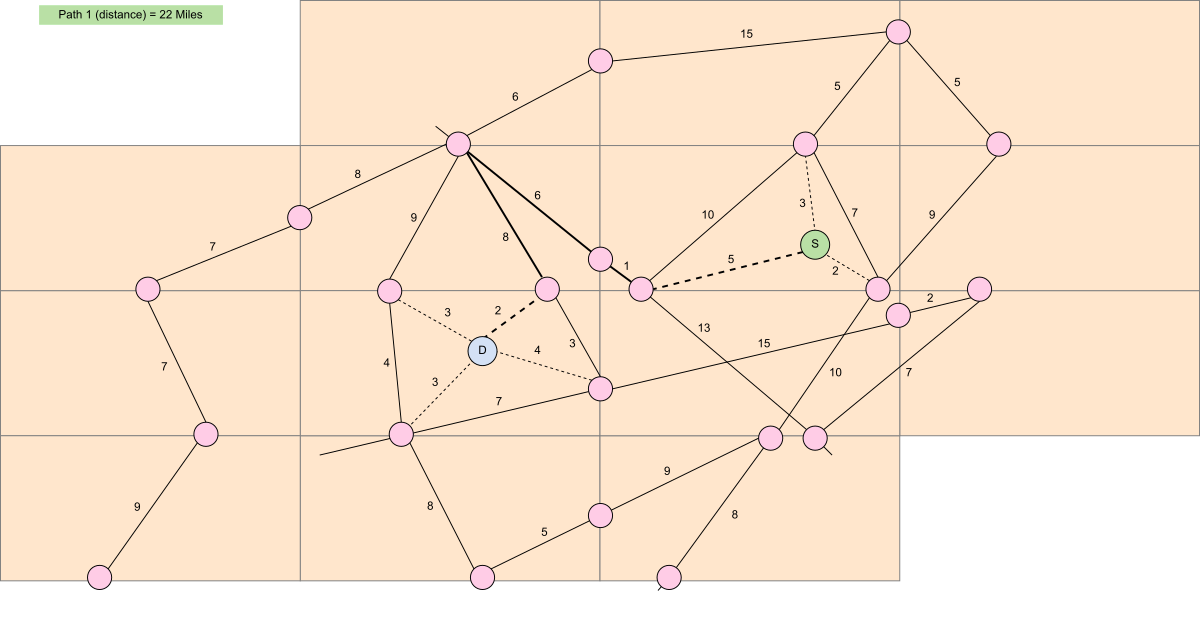
\includegraphics[width=\textwidth]{Images/chapter_28/section_4659727862071296/5631560120532992.png}
 \caption{We’ll start to find all the possible paths from S to D. One of the paths is highlighted in bold. The distance is calculated as 22 miles}
 \end{subfigure}
\end{figure}

\begin{figure}[htbp]
 \centering
 \begin{subfigure}[b]{0.48\textwidth}
 \centering
 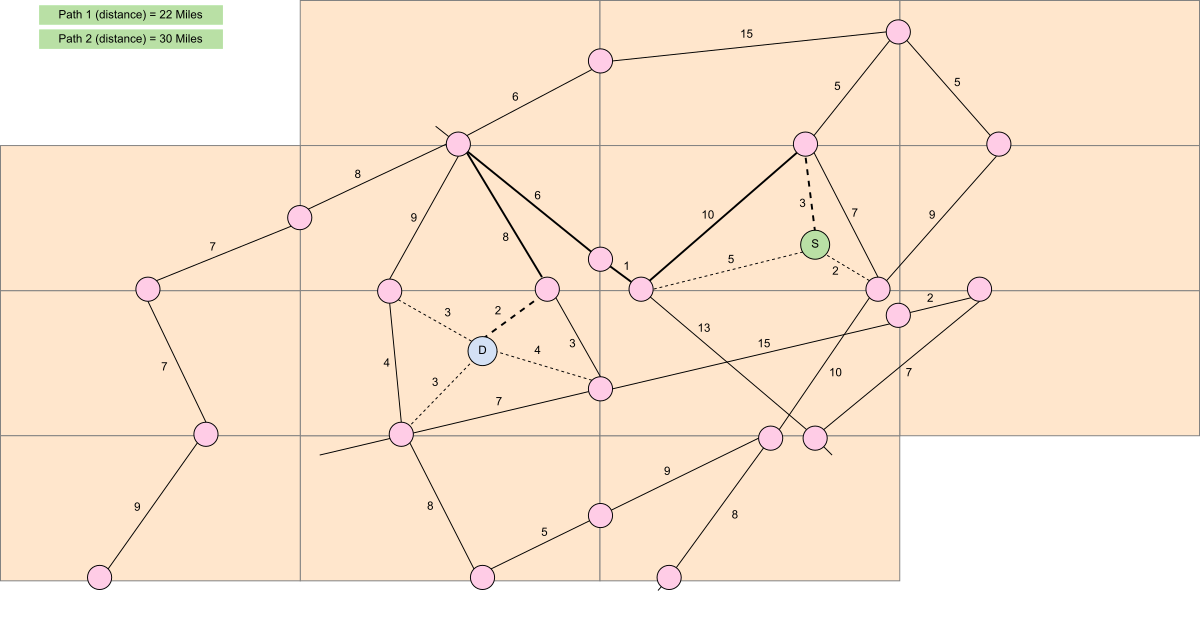
\includegraphics[width=\textwidth]{Images/chapter_28/section_4659727862071296/6140628870365184.png}
 \caption{Another path found that is 30 miles long}
 \end{subfigure}
 \hfill
 \begin{subfigure}[b]{0.48\textwidth}
 \centering
 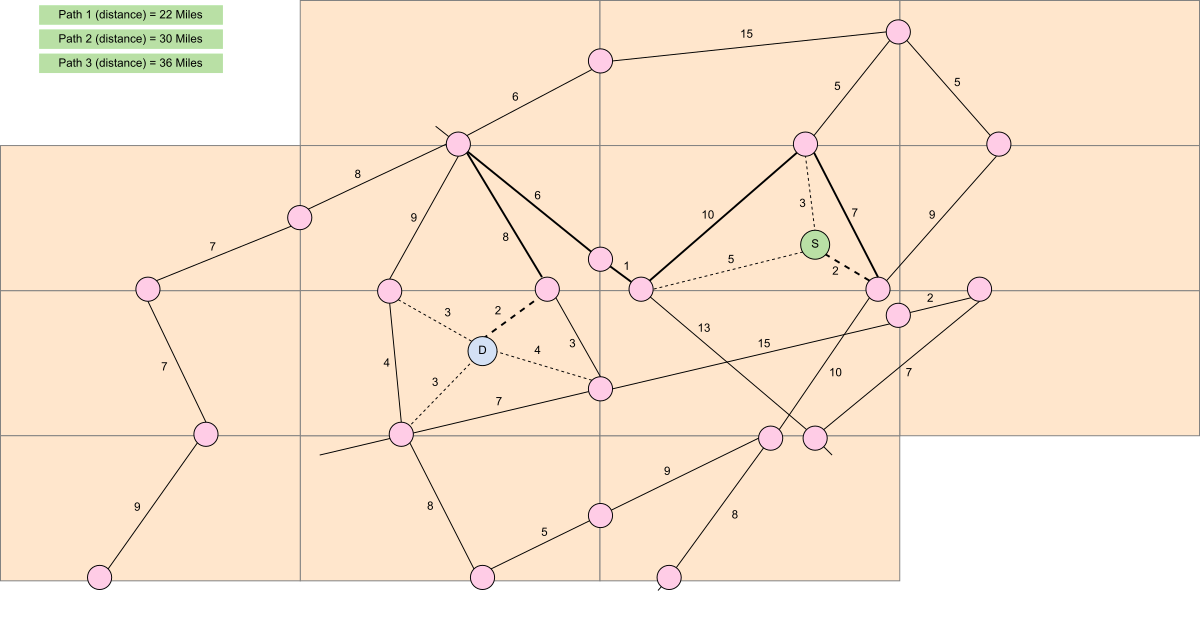
\includegraphics[width=\textwidth]{Images/chapter_28/section_4659727862071296/4795711669665792.png}
 \caption{Another path found that is 36 miles long}
 \end{subfigure}
\end{figure}

\begin{figure}[htbp]
 \centering
 \begin{subfigure}[b]{0.48\textwidth}
 \centering
 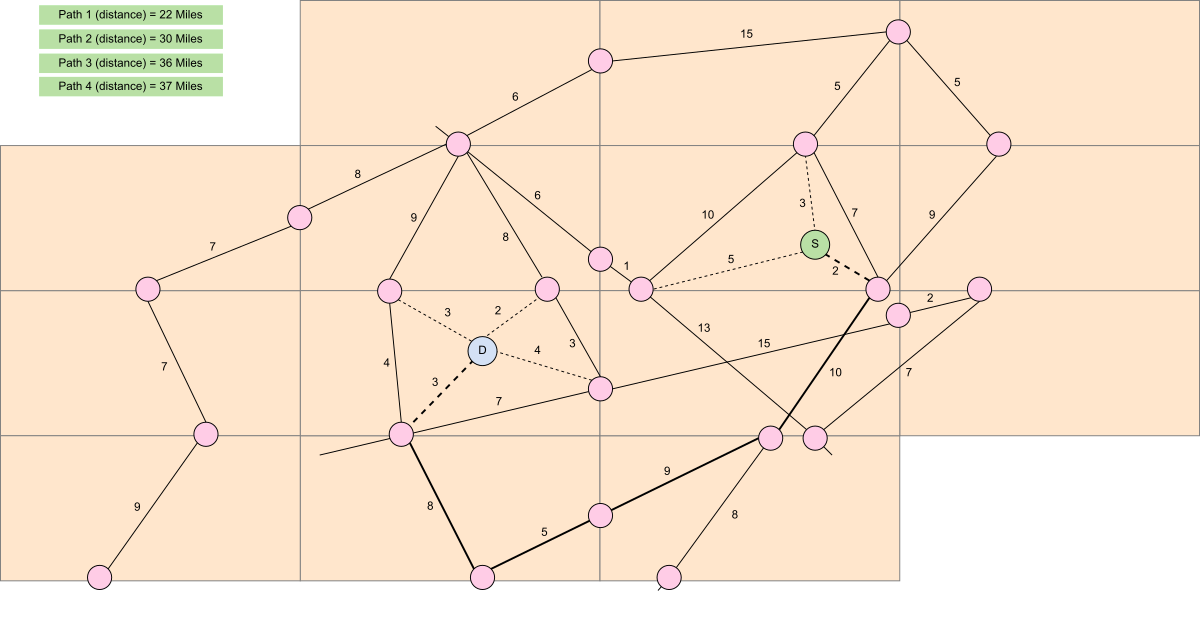
\includegraphics[width=\textwidth]{Images/chapter_28/section_4659727862071296/6337501279289344.png}
 \caption{Another path found that is 37 miles long}
 \end{subfigure}
 \hfill
 \begin{subfigure}[b]{0.48\textwidth}
 \centering
 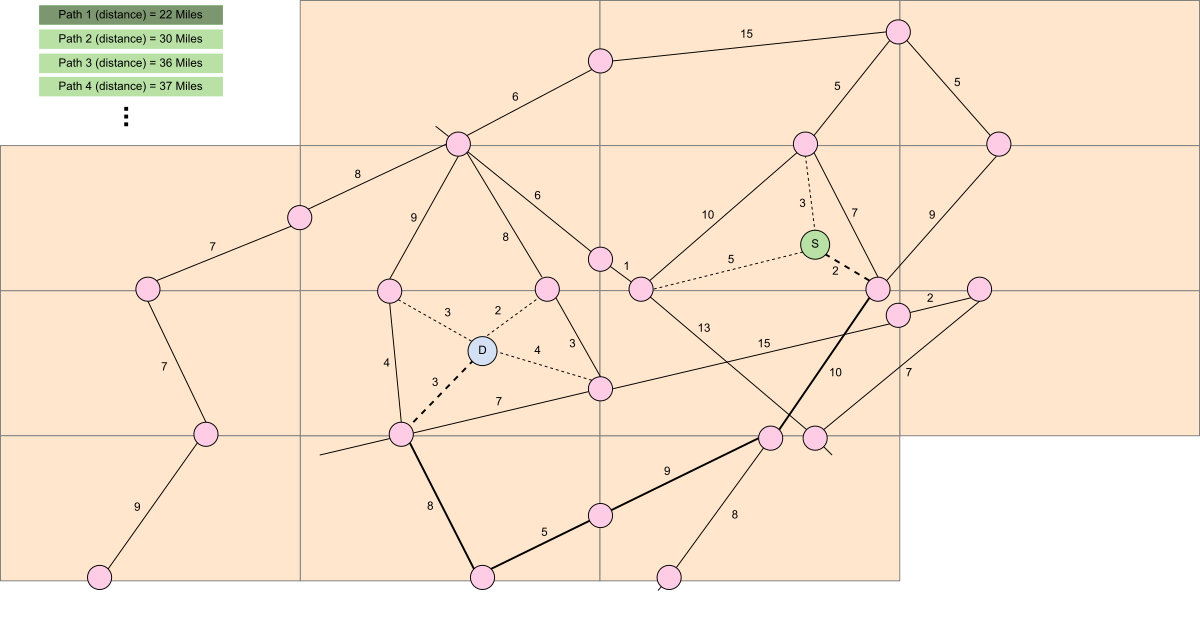
\includegraphics[width=\textwidth]{Images/chapter_28/section_4659727862071296/6591949368983552.png}
 \caption{We will keep on finding the possible paths and return the shortest path to the user}
 \end{subfigure}
\end{figure}

Let's summarize how we met the challenge of scalability. We divided our problem so that instead of working on a large road network as a whole, we worked on parts (segments) of it. The queries for a specific part of the road network are processed on that part only, and for the queries that require processing more than one part of the network, we connect those parts, as we have shown above.

\subsubsection{ETA computation}\label{6e-xFOcV1qVLXpD1xLZaN}
\\
For computing the ETA with reasonable accuracy, we collect the live location data ((userID,\ timestamp,(latitude,\ longitude))) from the navigation service through a pub-sub system. With location data streams, we can calculate and predict traffic patterns on different roads. Some of the things that we can calculate are:

\begin{itemize}
\item
\protect\phantomsection\label{C1apgQr9MX4jqo3mB0rDz}
Traffic (high/medium/low) on different routes or roads.
\item
\protect\phantomsection\label{ME_3B1avdGHW7yn7SaU9k}
The average speed of a vehicle on different roads.
\item
\protect\phantomsection\label{4uoyukmKbpEL1qgpt7LSO}
The time intervals during which a similar traffic pattern repeats itself on a route or road. For example, highway X will have high traffic between 8 to 10 AM.
\end{itemize}
\\
The information above helps us provide a more accurate ETA. For example, if we know that the traffic will be high at a specific time on a particular road, the ETA should also be greater than usual.
\\
In this lesson, we looked at how we meet the scalability challenge through segments and ETA computation using live data. In the next lesson, we'll discuss the design in more detail.

% End of section content